\section{Experiment Results}
We have conducted experiments on three datasets, where each dataset is obtained by monitoring 24-hour activities of two adults in a house through RFID.
The dataset comprises of events which are timestamped room occupancy data points. For instance, an event can correspond to person 1 being in the kitchen at 7:00 am. The summary of these three datasets is shown in table~\ref{tab_dataset}. 
\begin{table}[h]
\centering
\caption {Datasets summary.} \label{tab_dataset}
%\vspace{0.2cm}
\begin{tabular} {|l|l|c|}
\hline
Dataset  & Period & Number of people \\
\hline
study10 & 12 days & 2 \\
\hline
study11 & 10 days & 2 \\
\hline
study14 & 13 days & 2 \\
\hline
\end{tabular}
%\end{center}
%\end {table}
%\end{minipage}%
\end{table}
Study10 spans 12 days from 02/10/2014 to 02/21/2014 and Study11 spans 10 days from 01/29/2014 to 02/07/2014, and Study14 spans 13 days from 12/09/2013 to 12/21/2013.

We define \textit{unoccupancy} of a person as follows: 1) the person leaves the {\em outside-front} or {\em outside-back} for more than 30 minutes; 2) the person stays in the living room or dining room for more than 9 hours without any other activities; 3) the gap between any two events is more than 30 minutes. 
Since our research goal is to automate the turning on and off of the HVAC system at least 30 minutes before occupancy, the first and third constraints are in place. We are only interested in events where the {\em unocupancy} period is for an extended duration (> 30 minutes). The second constraints comes from our observation that if a person stays in one room for more than 9 hours without moving to other rooms, 
usually it means that the person goes out by leaving the RFID equipment at home. 
We delete events with duration less than 
2 minutes since these correspond to the individual walking back and forth across rooms and generally do not contribute to meaningful episodes. We conduct three types of experiments to compare three approaches, 
kNN, mixture EGH and Probability Density Function (PDF). 
For each dataset, we use $2/3$ data for training and the left $1/3$ for test. 
Following the approach in~\cite{scott2011preheat},
we organize one day's date into 96 15-minutes. 
For test data, we assume that we only know partial number of 15-minutes' chunks. Our target is to predict the occupancy in the rest of the day, or 30-minutes ahead. 

\subsection{Occupancy Prediction of Individuals}
%We apply three approaches, kNN, PDF based and mixture EGH time prediction model. 
%Similar to \cite{scott2011preheat},
%we organize one day's date into 96 15-minutes intervals with mixture EGH model. 
%Then we split the test date into three phases: 
%(1) before getting up, (2) after getting up and before going out, 
%(3) after going out and before coming back. 
%Thus our problem becomes to predict when the person going out 
%and when the person comes back. 
%Corresponding to these four phases, we adopt three different approaches. 
%For stage (1), the probability density function of going out and combing back event is calculated. 
%For stage (2), a duration-constraint episode mining and episode generative HMM is applied. 
%For stage (3), the probability density function of backing time based on 
%the time-constrains going out time is computed. 

%The results are shown in Figure~\ref{fig_study10} and Table~\ref{tab_individualResults}
%Figure~\ref{fig_study11}, and Figure~\ref{fig_study14}. 
%Each of these figures 

\begin{table*}[t]
%\vspace{0.2cm}
\hfill
\begin{minipage}[t]{1.0\linewidth}%

\caption{Precision Recall F-measure Comparison of Individual and Whole House Occupancy Prediction.}
\label{tab_individualResults}
\begin{center}
\makebox[\textwidth]{
\begin{tabular} {|l|l|l|l|l|l|l|l|l|}
\hline
\multirow{2}{*}{Dataset}&\multirow{2}{*}{Date}&\multirow{2}{*}{Person} & \multicolumn{3}{|c|}{EGH}&\multicolumn{3}{|c|}{kNN}  \\
\cline{4-9}
&&& Precision & Recall &F-measure &Precision & Recall & F-measure  \\
\hline
\multirow{3}{*}{study10}  & 02/17/2014 & person2& \textbf{1.00} & \textbf{1.00}&\textbf{1.00} & 0.99 & 0.98 & 0.98\\
\cline{2-9}
& 02/19/2014 & person1& 0.98 & 0.99 &0.98&  \textbf{0.99} &  \textbf{0.99} &  \textbf{0.99} \\
\cline{2-9}
& 02/20/2014 & person2&  \textbf{0.93} &  \textbf{0.92} &  \textbf{0.92} & 0.92 & 0.91 & 0.90 \\
\cline{2-9}
& 02/20/2014 & person1&  \textbf{0.95}& \textbf{0.94} & \textbf{0.94} & 0.94	& 0.93 & 0.93 \\
\cline{2-9}
& 02/20/2014 & \textbf{whole-house}&  \textbf{0.92}& \textbf{0.92} & \textbf{0.91} & 0.91	& 0.89 & 0.91 \\
\hline
\hline
\multirow{3}{*}{study11}  & 02/04/2014 & person2& 0.93 & 0.93 & 0.92  & \textbf{0.95} & \textbf{0.95} & \textbf{0.95}\\
\cline{2-9}
& 02/04/2014 & person1& 0.93 & 0.93 & 0.92  & \textbf{0.95} & \textbf{0.95} & \textbf{0.95} \\
\cline{2-9}
& 02/05/2014 & person2&  \textbf{0.85} &  \textbf{0.92} &  \textbf{0.86} & 0.87 & 0.87 & 0.84 \\
\cline{2-9}
& 02/05/2014 & person1&  \textbf{0.84} &  \textbf{0.90} &  \textbf{0.84} & 0.79 & 0.90 & 0.80 \\
\cline{2-9}
& 02/04/2014 & \textbf{whole-house}&  \textbf{0.918}& \textbf{0.924} & \textbf{0.913} & 0.916	& 0.921 & 0.911 \\
\cline{2-9}
& 02/05/2014 & \textbf{whole-house}&  \textbf{0.90}& \textbf{0.84} & \textbf{0.84} & 0.88	& 0.81 & 0.81 \\
\hline
\end{tabular}
}
\end{center}
\end{minipage}%
%\hfill%
\end{table*}
The individual occupancy prediction results on datasets Study10 and Study11 are summarized in table~\ref{tab_individualResults}. 
In Study10 as to the occupancy prediction for person2 on 02/17/2014, the mixture EGH performs better than kNN. 
Also, mixture EGH outperforms kNN for both persons on 02/20/2014. 
However, for person1 on 02/19/2014, kNN works a little bit better. 
When checking the original date on this test date, 
we find that the activities on this date is very similar to the historical activities in the training data.
%\textbf{When checking the original data, we find that the date on that day is similar to the historical data. - need to rephrase}
This observation leads us to the conclusion that when the test data is very highly similar to the historical data, 
kNN approach sometimes performs a little better.  
In Study11, a mixture of EGHs gets higher precision, recall and F-measure score on 02/05/2014 but the opposite on 02/04/2014. 
We analyzed the original data to reason the kNN's better performance. This date is anomalous to normal pattern since both individuals slept late that day (after 12:00am).
Before sleep, person1 even stayed in the kitchen for around two hours. 
The frequent episode $KZ$, which represents 'kitchen-unoccupied', 
usually occurs in the morning time instead of midnight. 
But mixture EGH model still assumes that $KZ$ pattern 
happens during morning time, 
therefore the prediction results are not accurate. 
%\textbf{On the contrary, 
%kNN doesn't consider the 
%actual place inside the room. - need to rephrase}
Since kNN ignores this fine granular activity pattern at a house and only considers the occupancy status in the past most similar 5 days, its performance is better. 
Generally speaking, the mixture EGH helps predict when a person 
leaves home during the period of sleeping and leaving home and its 
performance is competitive to the kNN approach. 

We also conduct experiments for individuals' {\em rest-of-day} occupancy prediction at different time. 
\begin{figure}[h]
\centering
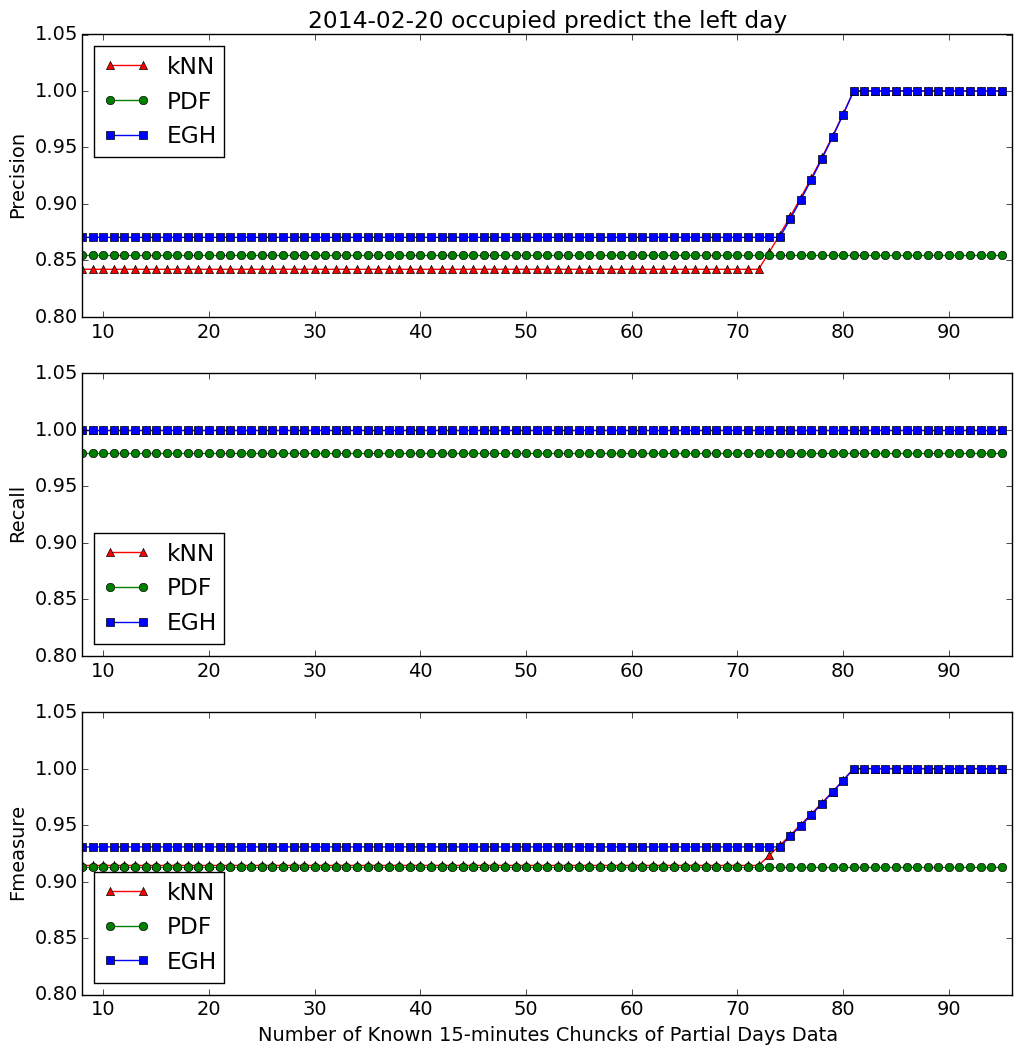
\includegraphics[width=1.0\textwidth]{adlfigs/study10person12014-02-20occupied.png}
\caption{Occupancy prediction precision, recall and f-measure comparison of three approaches 
of person1 on 02/20/2014 on Study10.}
\label{fig_study10}
\end{figure}
Figure~\ref{fig_study10} illustrates a person's occupancy prediction result on Study10.
There are three sub-figures. 
Each sub-figure describes the 
precision, recall, and f-measure 
of a person $person1$ on 02/20/2014. 
The blue line represents the mixture EGH model;
the green represents the PDF model;
the red denotes the kNN model. 
The x-axis is the number of known 15-minutes chunks of the test day. 
For instance, at $x=20$, 
we already know $20*15$ minutes' data 
and need to predict whether the in remaining $76$ chunks 
the home is occupied or not.
The y-axis denotes the precision, recall and f-measure values 
in the three sub-figures from top to down. 
The first sub-figure shows that  
the mixEGH has the highest precision, recall and F-measure on the test day 02/20/2014 
for occupancy prediction. The other two baseline approaches are comparable except that kNN performs better than PDF 
when the person comes back home after slot 72. 
Looking into the original data, we find that person1 actually comes later than usual 
in the training dataset. 
%In such case, mixture EGH performs best.  
%Figure \ref{fig_study10} (c) and (d) gives the occupancy and un-occupancy results 
%of person2 on 02/17/2014. 
%In such case, EGH mixture model performs best from the perspective of precision, recall and f-measure. 

\iffalse
Figure~\ref{fig_study14} (a) and (b) describe the case of person1 on 12/18/2013. 
Similar to Figure \ref{fig_study11} (a) and (b), 
mixture EGH model does not perform well before the person1 gets up 
and the reason keeps the same. 
The person1 slept late and some confused episodes are generated. 
Figure \ref{fig_study14} (c) and (d) describe the case of person1 on 12/19/2013. 
kNN performs better. Mixture EGH does not perform well because 12/19, 02/20 the person went out again after coming back and staying home for some time. However the training data don't include such case. 
\begin{figure}[h]
\centering
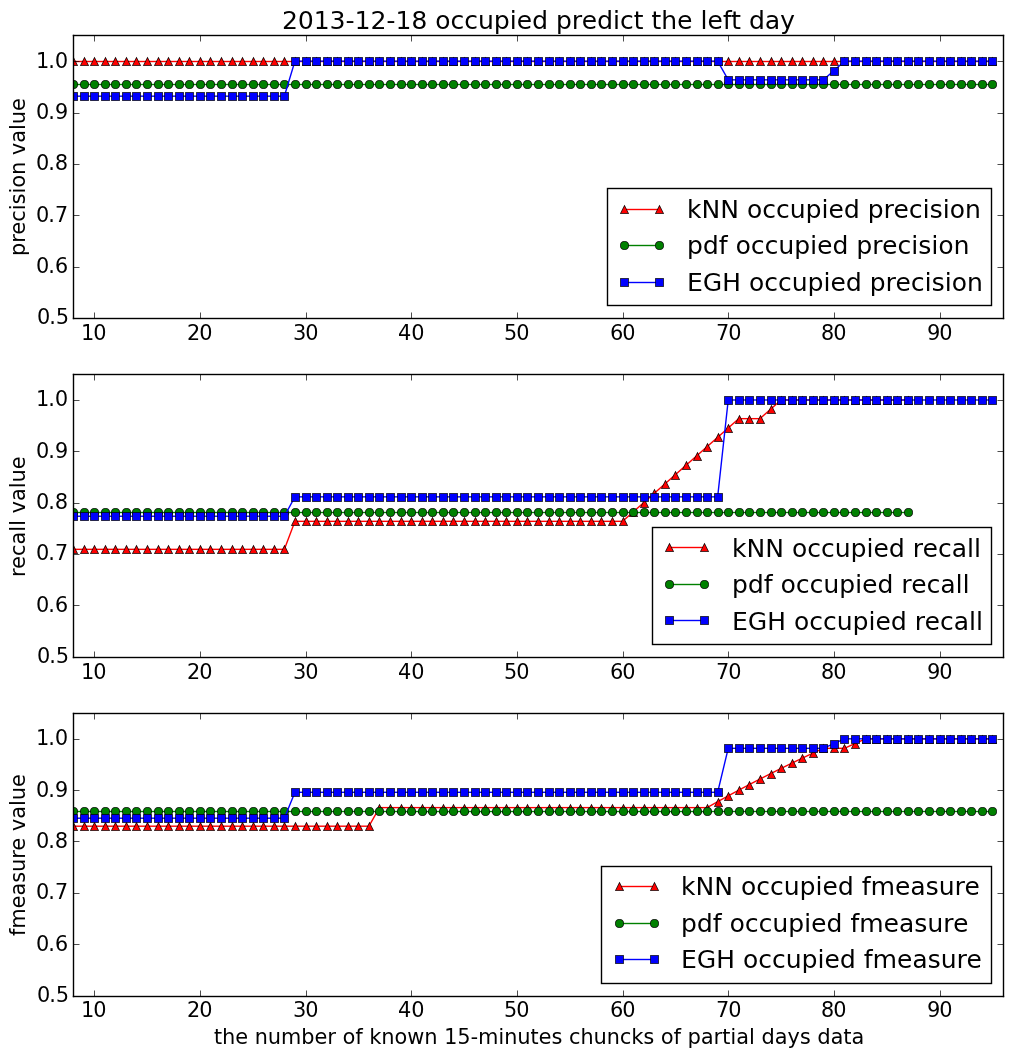
\includegraphics[width=0.5\textwidth]{adlfigs/study14person12013-12-18occupied.png} 
\caption{Study 14 Precision recall and f-measure comparison of three approaches.
person1 occupied 12/18/2014.}
\label{fig_study14}
\end{figure}
\fi


\subsection{Occupancy Prediction of Residential Buildings}
Based on individual prediction results, we deduce when a house is occupied
using logic OR operations on prediction results of two persons. 
The whole house occupancy prediction results are listed in 
table~\ref{tab_individualResults} and marked in bold. 
On Study10, the precision/recall/F-measure values of whole house are 0.92, 0.92 and 0.91, 
which are higher than the values from kNN approach 0.91, 0.90 and 0.91. Similarly mixture EGH model outperforms kNN in Study11. 
Note that in Study 11 on 02/04/2015, 
EGH does not perform as good as kNN on individuals
but performs a little bit better than kNN in occupancy prediction of the whole house. 
The reason behind that is because the actives of the two people inside home 
are not synchronized. The mixture EGH model can predict the 
occupancy for each person and grasp each person's activities more accurately. 
%When applying the logic OR operations on these two persons, 
%for whole-house occupancy prediction. 

\subsection{Limitations of Mixture EGH Model}
Although temporal mixture EGH model performs well on datasets Study10 and Study11, 
but not the same for the dataset Study14. 

\begin{table*}[!t]
%\vspace{0.2cm}
\hfill
%\begin{minipage}[t]{1.0\linewidth}%

\caption{Precision Recall F-measure of Individual and Whole House Occupancy Prediction in Study 14.}
\label{tab_resultsLimitation}
%\begin{center}
%\makebox[\textwidth]{
\centering
\small
\setlength\tabcolsep{2pt}
\begin{tabular} {|l|l|l|l|l|l|l|l|l|l|l|l|}
\hline
\multirow{2}{*}{Dataset}&\multirow{2}{*}{Date}&\multirow{2}{*}{Person} & \multicolumn{3}{|c|}{EGH}&\multicolumn{3}{|c|}{kNN} & \multicolumn{3}{|c|}{SVM} \\
\cline{4-12}
&&& precision & recall &fmeasure &precision & recall & fmeasure &precision & recall & fmeasure  \\
\hline
\multirow{3}{*}{study14}  & 12/18/2013 & person2&  \textbf{0.91} &  \textbf{0.91} &  \textbf{0.89} & 0.87 & 0.87 & 0.84 & 0.73 & 0.77 & 0.71\\
\cline{2-12}
& 12/18/2013 & person1&  \textbf{0.92} &  \textbf{0.92} &  \textbf{0.91} & 0.90 & 0.90 & 0.89 & 0.73 & 0.76 & 0.71 \\
\cline{2-12}
& 12/19/2014 & person2& 0.86 & 0.86 & 0.85  & \textbf{0.90} & \textbf{0.90} & \textbf{0.88} & 0.73 & 0.76 & 0.71\\
\cline{2-12}
& 12/19/2014 & person1& 0.85 & 0.84 & 0.84  & \textbf{0.86} & \textbf{0.86} & \textbf{0.85} & 0.73 & 0.76 & 0.71 \\
\cline{2-12}
& 12/20/2014 & person2& 0.92 & 0.94 & 0.92  & \textbf{0.98} & \textbf{0.97} & \textbf{0.97} & 0.75 & 0.79 & 0.75 \\
\cline{2-12}
& 12/20/2014 & person1& 0.90 & 0.91 & 0.90  & \textbf{0.95} & \textbf{0.95} & \textbf{0.95} & 0.75 & 0.79 & 0.75\\
\cline{2-12}
& 12/18/2013 & \textbf{wholehouse}&  \textbf{0.91}& \textbf{0.91} & \textbf{0.90} & 0.88	& 0.88 & 0.86 & 0.75 & 0.72 & 0.70 \\
\cline{2-12}
& 12/19/2013 & \textbf{wholehouse} & 0.841	& 0.845 & 0.838&  \textbf{0.848}& \textbf{0.853} & \textbf{0.842} & 0.79 & 0.74 & 0.74 \\
\cline{2-12}
& 12/20/2013 & \textbf{wholehouse} & 0.92	& 0.90 & 0.90&  \textbf{0.94}& \textbf{0.93} & \textbf{0.93} & 0.74 & 0.72 & 0.70 \\
\hline
\end{tabular}
%}
%\end{center}
%\end{minipage}%
%\hfill%
\end{table*}
Table~\ref{tab_resultsLimitation} shows that, 
in Study14, 
the mixture EGH model works better for the individual and whole-house occupancy prediction 
only on 12/18/2013 but not on 12/19/2013 and 12/20/2013. 
We check the activities of both individuals on these two days 
and find that both of them went out again 
after coming back and staying home for a while.
Since the episode of going out after coming back home from work 
do not occur frequently, mixture EGH cannot detect this pattern. Thus the occupancy prediction probability of these events 
is completely missing. However kNN performs better because it leverages all the 
historical data therefore, even if the abnormal event occurs once, 
this prediction approach incorporates it and obtains the average value. 

To relax the limitation of abnormal events, 
we propose a hybrid model for prediction:
when deploying this occupancy prediction in reality, 
for example for 30 minutes ahead prediction, 
just 15 minutes before prediction, if a person goes out again after coming back, 
the deployed system switches to the kNN approach other than mixture EGH model for prediction. In such case, this hybrid model can always get the best prediction results. 

\subsection{30 minutes Ahead House Occupancy Prediction with Hybrid Approach}
Preheating the house needs to evaluate how much time in advance to automatically turn on/off HVAC and the advance notice time estimation is given in~\cite{scott2011preheat}. 
Here we use 30 minutes ahead of time house occupancy prediction. 
%because it is reasonable for preheating. 
We compare the ROC curve of three approaches: mixture EGH model, kNN, and a hybrid approach of mixture EGH model and kNN. 
In this hybrid approach, 
we set mixture EGH results as the baseline, 
then replace the values of the mixture model by the values from kNN model 
in the following two situations: 
1) after a person comes back home; 2) the prediction probability of kNN is greater than 0.8. 
Figure~\ref{fig_rocresults_1}, ~\ref{fig_rocresults_2},~\ref{fig_rocresults_3}, illustrates the ROC curve of the whole house occupancy prediction on 02/20/2014 of dataset Study10, 02/04/2014 of dataset Study 11 
and 12/20/2013 of dataset Study14. 
The red and green represents the kNN and mixture EGH model, 
the blue denotes the hybrid approach. 
The ROC curves show that the hybrid approach always hold the largest area, namely 
0.96, 0.92 and 0.92, 
which indicate that the hybrid approach always performs the best. 
%\begin{figure*}[t]
	\centering{
		\begin{tabular}{cccc}		
		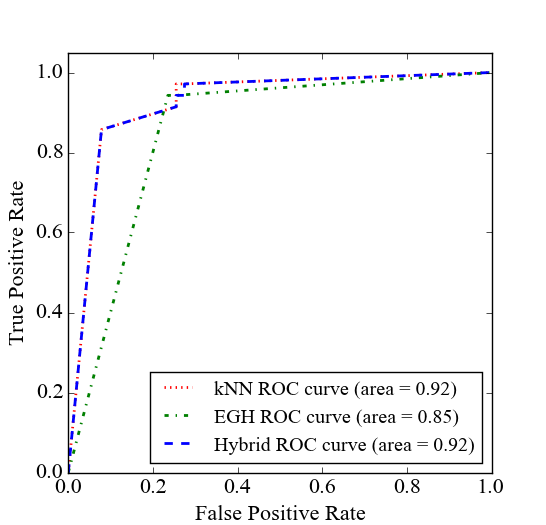
\includegraphics[width=0.33\textwidth]{adlfigs/study10ROC_02202014.png} &
		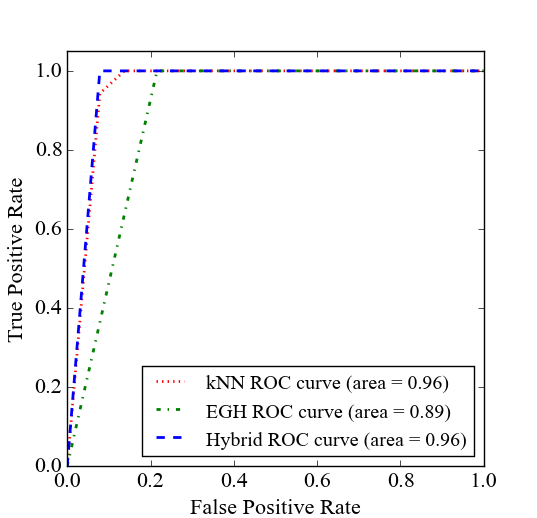
\includegraphics[width=0.33\textwidth]{adlfigs/study11ROC_02042014.png} &
		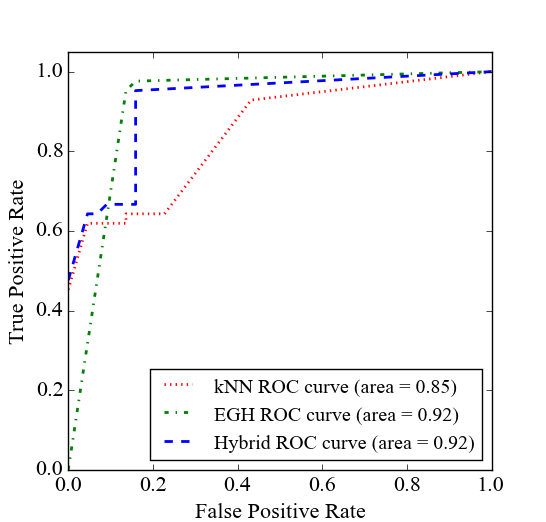
\includegraphics[width=0.33\textwidth]{adlfigs/study14ROC_12202013.png}
		\tabularnewline
		(a)&(b)&(c) \tabularnewline
		\end{tabular}
		}
	\caption{
	ROC curve of house occupancy prediction on 
(a) Study10 (02/20/2014). (b) Study11 (02/04/2014). (c) Study14 (12/20/2013).
}
	\label{fig_rocresults}
\end{figure*}
\begin{figure}[h]
	\centering{
		\begin{tabular}{cccc}		
		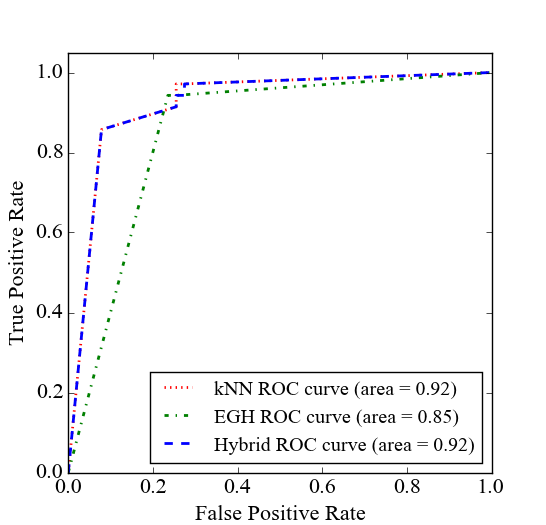
\includegraphics[width=0.7\textwidth]{adlfigs/study10ROC_02202014.png} &
		\tabularnewline
		(a)\tabularnewline
		\end{tabular}
		}
	\caption{
	ROC curve of house occupancy prediction on Study10 (02/20/2014).}
	\label{fig_rocresults_1}
\end{figure}

\begin{figure}[h]
	\centering{
		\begin{tabular}{cccc}		
		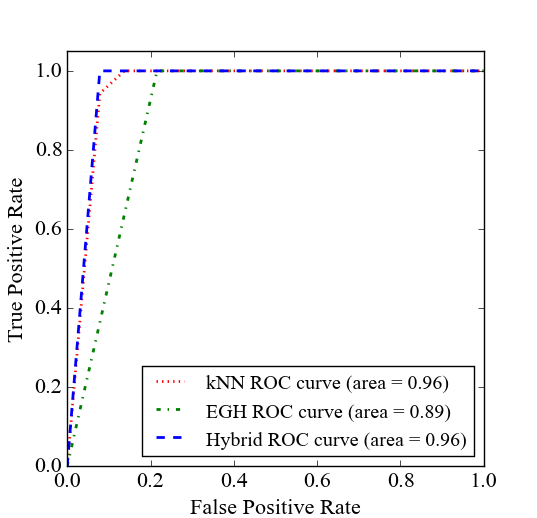
\includegraphics[width=0.7\textwidth]{adlfigs/study11ROC_02042014.png} &
		\tabularnewline
		((b)\tabularnewline
		\end{tabular}
		}
	\caption{
	ROC curve of house occupancy prediction on Study11 (02/04/2014).
}
	\label{fig_rocresults_2}
\end{figure}

\begin{figure}[h]
	\centering{
		\begin{tabular}{cccc}		
		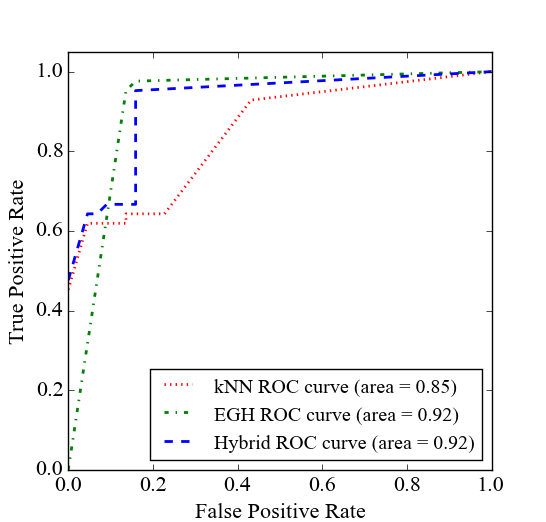
\includegraphics[width=0.7\textwidth]{adlfigs/study14ROC_12202013.png}
		\tabularnewline
		(c) \tabularnewline
		\end{tabular}
		}
	\caption{
	ROC curve of house occupancy prediction on (c) Study14 (12/20/2013).
}
	\label{fig_rocresults_3}
\end{figure}


%Also, we compare the 30 minutes whole house precision/recall/f-measure with the ROC curve, 
%the kNN ROC has a larger area even if EGH approach performs better on study10 and study11. 

%It depicts that ROC curve of mixture EGH model occupied larger area 0.92 than that from kNN approach 0.85. 
%We observe that although the precision/recall/fmeasure values are very close as in table~\ref{tab_individualResults}. 
%This hints that although the precision/recall/fmeasure results are competitive, 
%mixture EGH model can separate the occupancy and un-occupancy more sharply. 



%There are three test days in the dataset study14, 
%EGH outperforms kNN on the first day. 
%It's a tie on the second day. 
%The only exception on these datasets is the last day's experiment on study14, 
%kNN performs better because EGH mixture model currently
%only works on one-time even prediction. 


